\documentclass[a4paper, 12pt]{article}
\usepackage[a4paper, top = 1.5cm, bottom = 1.5cm, left = 1cm, right = 1cm]{geometry}
\usepackage[english, russian]{babel}
\usepackage{graphicx}
\usepackage{subcaption}
\usepackage{mathtools}
\usepackage{amsfonts}
\usepackage{float}
\title{Лабораторная работа № 4.8А "Резонанс токов"}
\author{Кирилл Шевцов Б03-402}
\date{16.10.2025}
\begin{document}
\maketitle
\section*{Лабораторная установка}
\begin{figure}[htbp]
    \centering
    \includegraphics[width=0.7\linewidth]{equip.png}
    \label{Лабораторная установка}
    \caption{Лабораторная установка}
\end{figure}
Задание предполагает снятие зависимости значений тока на учасках с амперметрами от индуктивности катушки.
Согласно установке : амперметр $A_{1}$ показывает общий ток в цепи, $A_{2}$ - ток на участке с катушкой, $A_{3}$ - ток на конденсаторе заданной
заданной емкости $C = 120$ мкФ.\newline
Напряжение подается от сети постоянным $U = 220$ В, частота генератора также постоянна и равна $\nu = 50$ Гц.\newline
Картину резонанса можно увидеть либо по минимальному току на амперметре $A_{1}$, либо на осциллорафе: резонансу соответсвует нулевой сдвиг фазы,
то есть вырождение эллипса в наклонную прямую.\newline
Резонанс токов полагается исследовать на параллельном колебательном контуре, поскольку напряжение на участках цепи, параллельных включенному
вольтметру, совпадают.
\section*{Измерения и результаты}
\begin{enumerate}
    \item Резонанс токов для частоты $\nu = 50$ Гц. (рисунок \ref{resonanse})
    \begin{figure}[htbp]
        \centering
        \begin{subfigure}{0.3\textwidth}
            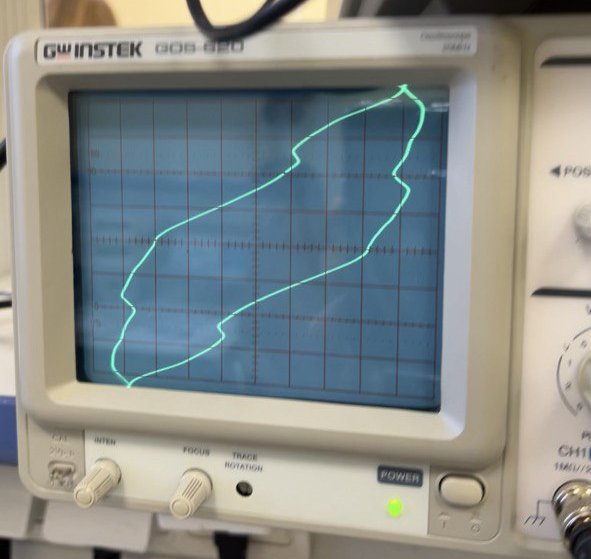
\includegraphics[width=\textwidth]{ellipse.jpg}
            \caption{до резонанса}
            \label{ellipse}
        \end{subfigure}
        \qquad
        \begin{subfigure}{0.3\textwidth}
            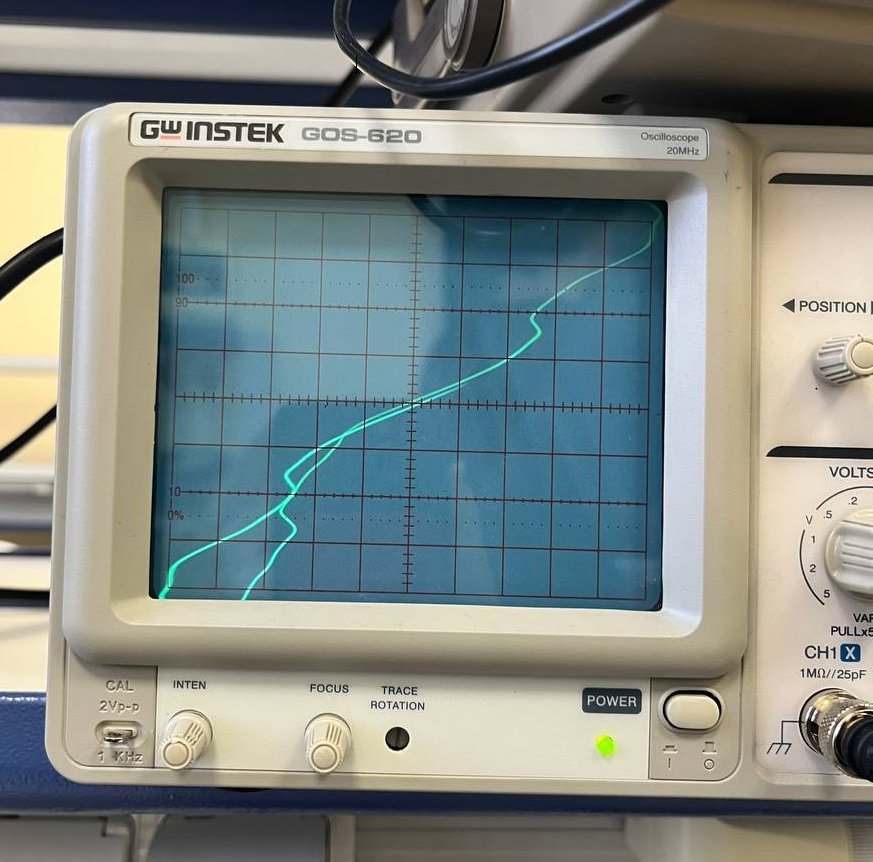
\includegraphics[width=\textwidth]{resonanse.jpeg}
            \caption{резонанс}
            \label{resonanse}
        \end{subfigure}
        \caption{Показания на экране осциллографа}
        \label{fig:figures}
    \end{figure}
    \item Будем медленно вдвигать сердечник в катушку индуктивности. Зафиксировав расстояние, на которое вдвинут сердечник, снимем показания
    амперметров $A_{1}$, $A_{2}$, $A_{3}$. Ток на учатках с катушкой, кондесатором и общий ток обозначим соответсвенно $I_{L}$, $I_{C}$, $I$.
    \begin{table}[htbp]
        \centering
        \begin{tabular}{|c|c|c|c|c|c|c|c|c|c|c|c|}
            \hline
            $x$, см & 7.0 & 6.5 & 6.0 & 5.5 & 5.0 & 4.5 & 4.0 & 3.5 & 3.0 & 2.5 \\
            $I_{L}$, А & 0.417 & 0.387 & 0.354 & 0.325 & 0.301 & 0.277 & 0.255 & 0.233 & 0.213 & 0.186 \\
            $I_{C}$, А & 0.401 & 0.395 & 0.392 & 0.393 & 0.386 & 0.398 & 0.395 & 0.395 & 0.398 & 0.391 \\
            $I$, А & 0.05 & 0.045 & 0.056 & 0.078 & 0.100 & 0.125 & 0.144 & 0.164 & 0.186 & 0.207 \\
            \hline
        \end{tabular}
        \caption{снятие токов при вдвижении сердечника}
        \label{снятие токов при вдвижении сердечника}
    \end{table}\newline
    Обозначим четкий диапазон перемещения дросселя $\Delta = 1.5 \div 6.9$ см.
    Напряжение на ЛАТР поддерживаем постоянным и равным $U_{0} = (10 \pm 1)$ В.
    Частота лабораторного трансформатора $\omega = (50\pm 10)$ Гц.
    Емкость конденсатора $C = (120\pm 10)$ мкФ.
    \newpage
    \item Построим графики зависимостей сил тока на рассмотренных участках от положения $x$ сердечника.
    (по горизонтальной оси - расстояние, на которое сердечник выдвинут из катушки)
    \begin{figure}[htbp]
        \centering
        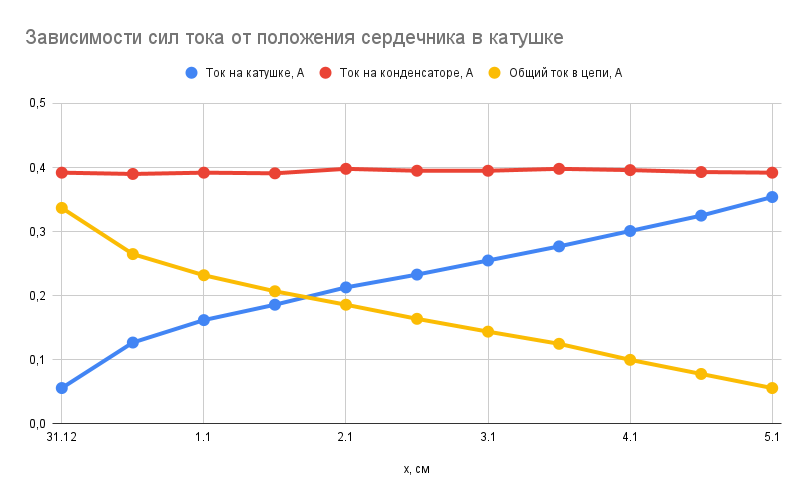
\includegraphics[width=0.6\linewidth]{I_x.png}
        \label{зависимость сил тока для разных расстояний}
        \caption{зависимость силы тока от положения сердечника в катушке}
    \end{figure}\newline
    Из результатов измерений видно, что сила тока на учатке с катушкой постоянно увеличивается, общий ток в цепи уменьшается. Сила тока 
    на участке с конденсатором остается постоянной, поскольку она зависит только от частоты и напряжения генератора.
    \begin{equation}
        I_{C} = U_{0} \omega C = 2\pi \nu C U_{0} = 0.37\pm 0.01\ \text{A}
        \label{ток на участке с конденсатором}
    \end{equation}
    И последние два определяются соотношением
    \begin{align}
        I_{L} = \frac{U_{0}}{\sqrt{(r_{L})^{2} + (\omega_{0}L)^{2}}}, \quad I = I_{L} + I_{C}
    \end{align}
    \item Резонансные значения тока на рассматриваемых участках цепи.
    \begin{table}[H]
        \centering
        \begin{tabular}{|c|c|c|c|c|c|}
            \hline
            $I^{res}_{L}$, А & $I^{res}_{C}$, А & $I^{res}$, А & $\Delta I^{res}_{L}$, А & $\Delta I^{res}_{C}$, А & $\Delta I^{res}$, А\\
            \hline
            0.428 & 0.419 & 0.049 & \multicolumn{3}{|c|}{0.001}\\
            \hline
        \end{tabular}
        \caption{резонансные токи на катушке, конденсаторе и в цепи}
        \label{резонансные токи на катушке, конденсаторе и в цепи}
    \end{table}
    \item Рассчитаем добротность колебательного контура - через токи, и резонансное сопротивление - через полный ток и напряжение.
    \begin{align}
        Q &= \frac{I^{res}_{C}}{I^{res}} = \frac{0.428}{0.049} = 8.73 \pm 0.19, \quad \Delta Q = Q\left(\frac{\Delta I^{res}_{C}}{I^{res}_{C}} + \frac{\Delta I^{res}}{I^{res}}\right) = 0.022Q = 0.19\\
        R_{\Sigma} &= \frac{U_{0}}{I^{res}} = \frac{10.00}{0.049} = 204.08 \pm 24.37\ \text{Ом}, \quad \Delta R_{\Sigma} = R_{\Sigma}\left(\frac{\Delta U_{0}}{U_{0}} + \frac{\Delta I^{res}}{I^{res}}\right) = 0.12R_{\Sigma} = 24.57\ \text{Ом}
    \end{align}
    \item Рассчитаем индуктивность катушки $L_{res}$ через емкость и частоты $\nu = 50$ Гц и $\nu = 1000$ Гц, а затем через добротность и емкость сделаем рассчет активного
    сопротивления катушки. Расчет для частоты $\nu = 50$ Гц.
    \begin{align}
        L_{res} = \frac{1}{\omega^{2}C} = 0.083\pm 0.024\ \text{Гн}, \quad
        \Delta L_{res} = L_{res}\left(\frac{2\Delta \omega}{\omega} + \frac{\Delta C}{C}\right) = 0.28L_{res} = 0.024\ \text{Гн}\\
        r_L = \frac{\omega L_{res}}{Q} = 3.02\pm 0.49\ \text{Ом}, \quad
        \Delta r_L = r_L\left(\frac{\Delta L_{res}}{2L_{res}} + \frac{\Delta C}{C} - \frac{\Delta Q}{Q}\right) = 0.20r_{L} = 0.63\ \text{Ом}
    \end{align}
    Расчет для частоты $\nu = 1000$ Гц.
    \begin{align}
        L_{res} = \frac{1}{\omega^{2}C} = 0.21\pm 0.06\ \text{мГн}, \quad
        \Delta L_{res} = L_{res}\left(\frac{2\Delta \omega}{\omega} + \frac{\Delta C}{C}\right) = 0.28L_{res} = 0.06\ \text{мГн}\\
        r_L = \frac{\omega L_{res}}{Q} = 0.15\pm 0.03\ \text{Ом},\quad
        \Delta r_L = r_L\left(\frac{\Delta L_{res}}{2L_{res}} + \frac{\Delta C}{C} - \frac{\Delta Q}{Q}\right) = 0.20r_{L} = 0.03\ \text{Ом}
    \end{align}
    \item Сравним полученные значения сопротивления и индуктивности со значениями, снятыми с моста $E7-8$ при частоте $\nu = 50$ и $\nu = 1000$ Гц.
    \begin{table}[htbp]
        \centering
        \begin{tabular}{|c|c|c|c|c|c}
            \hline
            Частота, Гц & \multicolumn{2}{|c|}{Расчет с E7-8} & \multicolumn{2}{|c|}{Расчет с формулами и графиками}\\
            \hline
            $\nu$, Гц & $L_{res}$, мГн & $r_{L}$, Ом &  $L_{res}$, мГн & $r_{L}$, Ом\\
            \hline
            $50$ & $67.011\pm 0.001$ & $1.937\pm 0.001$ & $83.00\pm 24.00$ & $3.02\pm 0.63$\\
            $1000$ & $60.610\pm 0.001$ & $31.850\pm 6.001$ & $0.21\pm 0.06$ & $0.15\pm 0.03$\\
            \hline
        \end{tabular}
        \caption{Сравнение с полученными данными}
        \label{Сравнение с полученными данными}
    \end{table}
    \item Угол между напряжением и током катушки (для частот 50 и 1000 Гц соответсвенно)
    \begin{align}
        z_{L} = r_{L} + j\omega L, \quad
        tg\psi = \frac{\omega L}{r_{L}} = 8.63, \quad \psi = \arctan\frac{\omega L}{r_{L}} = 83.3^{\circ}\\
        z_{L} = r_{L} + j\omega L, \quad
        tg\psi = \frac{\omega L}{r_{L}} = 8.79, \quad \psi = \arctan\frac{\omega L}{r_{L}} = 83.5^{\circ}
    \end{align}
    Иначе, напряжение опережает ток на катушке на 90 градусов (если элементы идеальные).
    Составляющие напряжения на катушке (для частот 50 и 1000 Гц).
    \begin{align*}
        U_{L_{act}} = U_{0} \cdot \cos \psi = 10 \cdot 0.1166 = 1.166\text{ В}, \quad
        U_{L_{react}} = U_{0} \cdot \sin \psi = 10 \cdot 0.9931 = 9.931\text{ В}
    \end{align*}
    Для тока на конденсаторе (Аналогично для частот 50 и 1000 Гц)
    \begin{align}
        z_{C} = -\frac{j}{\omega L}, \quad tg\psi = \frac{\omega L}{0} \rightarrow \infty, \quad \psi = -90^{\circ}, \quad I_{C} = 2\pi\nu CU_{0}
    \end{align}
    Иначе, сила тока на конденсаторе опережает по фазе на 90 градусов с напряжением на конденсаторе.
    Для тока на катушке и активном сопротивлении (для частот 50 и 1000 Гц).
    \begin{align}
        I_{act} = \frac{U_{act}}{r_{L}} = 0.37\ \text{А}, \quad I_{react} = \frac{U_{react}}{\omega L} = 0.381\ \text{А}, \quad I_{C} = 0.37\ \text{А}\\
        I_{act} = \frac{U_{act}}{r_{L}} = 7.44\ \text{А}, \quad I_{react} = \frac{U_{react}}{\omega L} = 7.474\ \text{А}, \quad I_{C} = 7.53\ \text{А}
    \end{align}
    Диаграмма токов (множитель масштаба равен 0.1, все измерения умножаются на 10)
    \begin{figure}[H]
        \centering
        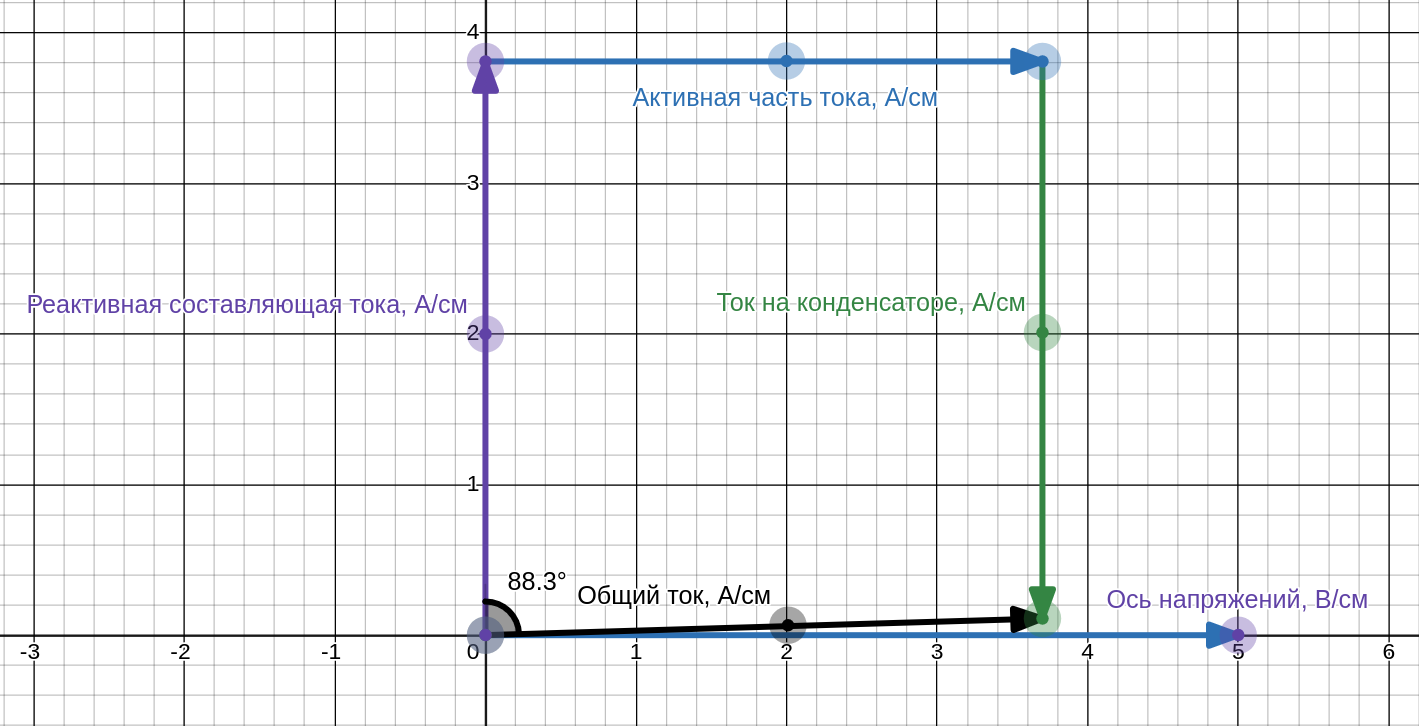
\includegraphics[width=0.7\linewidth]{i_diag.png}
        \label{треугольная векторная диаграмма}
        \caption{Векторная диаграмма для токов}
    \end{figure}
    Параметры катушки по графику (для частот)
    \begin{align}
        r_L = \frac{U_{L_{act}}}{{I_L}} = \frac{1.1166}{0.428} = 2,60\text{ Ом} \quad
        L = \frac{U_{L_{react}}}{\omega \cdot I_L} = \frac{9.931}{314.15 \cdot 0.428} = 0.074\text{ Гн}
    \end{align}
    \item Сравнительная таблица 
    \begin{table}[H]
        \centering
        \begin{tabular}{|c|c|c|c|c|c|c|c|}
            \hline
            Частота, Гц & \multicolumn{2}{|c|}{Расчет с E7-8} & \multicolumn{2}{|c|}{Расчет с графиками} & \multicolumn{2}{|c|}{Расчет с диаграммой}\\
            \hline
            $\nu$, Гц & $L_{res}$, мГн & $r_{L}$, Ом &  $L_{res}$, мГн & $r_{L}$, Ом & $L_{res}$, мГн & $r_{L}$, Ом\\
            \hline
            $50$ & $67.011\pm 0.001$ & $1.937\pm 0.001$ & $83.00\pm 24.00$ & $3.02\pm 0.63$ & $74\pm 10$ & $2.60\pm 0.01$\\
            $1000$, Гц & $60.01\pm 10.00$ & $31.850\pm 5.001$ & $0.21\pm 0.006$ & $0.15 \pm 0.03$ & - & -\\
            \hline
        \end{tabular}
        \caption{Параметры катушки, измеренные разными способами}
        \label{Параметры катушки, измеренные разными способами}
    \end{table}
\end{enumerate}
\section*{Вывод}
В работе были измерены зависимости силы тока на разных участках параллельного колебательного контура. 
Было показано, что при вдвижении сердечника в катушку ток на участке с конденсатором остается постоянным на протяжении всех измерений, и зависит лишь от напряжения ЛАТР и частоты генератора, на участке с катушкой все время уменьшается, поскольку при вдвижении в нее
сердечника индуктивность уменьшается.
Контур при резонансе токов удобно выбирать именно параллельным, поскольку необходимо удерживать постоянным только напряжение.
\end{document}